% fig_pinn_accuracy.tex
% TR-46: Per-class classification accuracy PINN vs Baseline
%
% Data from Study C:
%   Class    PINN%   Baseline%
%   MISS     85.19   81.48
%   87L      92.39   87.82
%   Z1       95.71   84.55
%   EXT      93.02   86.05

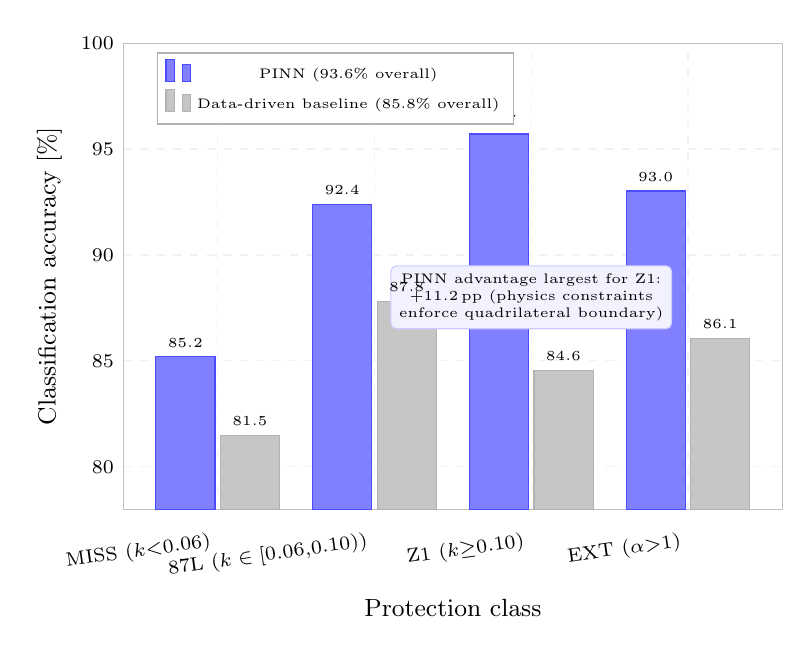
\begin{tikzpicture}
\begin{axis}[
  name         = accax,
  width        = 0.82\textwidth,
  height       = 7.5cm,
  ybar,
  bar width    = 0.75cm,
  xlabel       = {Protection class},
  ylabel       = {Classification accuracy [\%]},
  xlabel style = {font=\small},
  ylabel style = {font=\small},
  ymin=78, ymax=100,
  ytick        = {80,85,90,95,100},
  yticklabel style={font=\scriptsize},
  xtick        = {1,2,3,4},
  xticklabels  = {MISS ($k{<}0.06$),
                  87L ($k\in[0.06{,}0.10)$),
                  Z1 ($k{\geq}0.10$),
                  EXT ($\alpha{>}1$)},
  xticklabel style={font=\scriptsize, rotate=8, anchor=north east},
  tick style   = {draw=none},
  axis line style={gray!50},
  grid         = major,
  grid style   = {gray!10, dashed},
  nodes near coords,
  nodes near coords style={font=\tiny, anchor=south},
  every node near coord/.append style={
    /pgf/number format/.cd, fixed, fixed zerofill, precision=1
  },
  legend style={at={(0.05,0.98)}, anchor=north west, font=\tiny,
                draw=gray!60, fill=white},
  enlarge x limits=0.20,
  clip=false,
]

%% PINN bars (blue)
\addplot[fill=blue!50, draw=blue!70]
  coordinates {(1,85.19) (2,92.39) (3,95.71) (4,93.02)};
\addlegendentry{PINN (93.6\% overall)}

%% Baseline bars (gray)
\addplot[fill=gray!45, draw=gray!60]
  coordinates {(1,81.48) (2,87.82) (3,84.55) (4,86.05)};
\addlegendentry{Data-driven baseline (85.8\% overall)}

%% PINN advantage annotation
\node[draw=blue!20, fill=blue!5, rounded corners=2pt,
      font=\tiny, inner sep=3pt, align=center]
  at (axis cs:3, 88)
  {PINN advantage largest for Z1:\\
   $+11.2$\,pp (physics constraints\\
   enforce quadrilateral boundary)};

\end{axis}
\end{tikzpicture}
